\documentclass[pdftex]{beamer} 

\setbeamertemplate{navigation symbols}{} % выключить навигационную панльку
\setbeamertemplate{footline}[frame number] % нумерация страниц

\usepackage{graphicx}
\usepackage{amsmath,amssymb,amsthm} 
\usepackage{pb-diagram}
\usepackage{ucs}
\usepackage[utf8x]{inputenc}
\usepackage[russian]{babel}
\usepackage{epstopdf}
\usepackage{multicol}
\usepackage{cancel}
\usepackage{hyperref}
\usepackage{amsfonts}

\usepackage{listings}
\usepackage{textcomp}
\definecolor{listinggray}{gray}{0.9}
\definecolor{lbcolor}{rgb}{0.9,0.9,0.9}
\lstset{
%	backgroundcolor=\color{lbcolor},
        language=Mathematica,
	tabsize=2,
	rulecolor=,
        basicstyle=\scriptsize,
        upquote=true,
%        aboveskip={1.5\baselineskip},
        columns=fixed,
        showstringspaces=false,
        extendedchars=true,
%        breaklines=true,
        prebreak = \raisebox{0ex}[0ex][0ex]{\ensuremath{\hookleftarrow}},
%        frame=single,
        showtabs=false,
        showspaces=false,
        showstringspaces=false,
        identifierstyle=\ttfamily,
        keywordstyle=\color[rgb]{0,0,1},
        commentstyle=\color[rgb]{0.133,0.545,0.133},
        stringstyle=\color[rgb]{0.627,0.126,0.941},
}

%%%%%%%%%%%%%%%%%%%%%%%%%%%%%%%%%%%%%%%%%%%%%%%%%%%%%%%%%%%%%%%%%%%%%%%%%%%%%%%%%%%%%%%%%%%%%%%%%%%

%\newtheorem{theorem}{Theorem}
%% \newtheorem{acknowledgement}[theorem]{Acknowledgement}
%% \newtheorem{algorithm}[theorem]{Algorithm}
%% \newtheorem{axiom}[theorem]{Axiom}
%% \newtheorem{case}[theorem]{Case}
%% \newtheorem{claim}[theorem]{Claim}
%% \newtheorem{conclusion}[theorem]{Conclusion}
%% \newtheorem{condition}[theorem]{Condition}
%% \newtheorem{conjecture}[theorem]{Conjecture}
%% \newtheorem{mycorollary}[theorem]{Corollary}
%% \newtheorem{mycriterion}[theorem]{Criterion}
%% \newtheorem{mydefinition}[theorem]{Definition}
%% \newtheorem{myexample}[theorem]{Example}
%% \newtheorem{myexercise}[theorem]{Exercise}
\newtheorem{mylemma}[theorem]{Лемма}
%% \newtheorem{mynotation}[theorem]{Notation}
%% \newtheorem{myproblem}[theorem]{Problem}
%% \newtheorem{myproposition}[theorem]{Proposition}
%% \newtheorem{myremark}[theorem]{Remark}
%% \newtheorem{mysolution}[theorem]{Solution}
%% \newtheorem{mysummary}[theorem]{Summary}
%% \newenvironment{myproof}[1][Proof]{\textbf{#1.} }{\ \rule{0.5em}{0.5em}}


\newcommand{\go}{\stackrel{\circ }{\mathfrak{g}}}
\newcommand{\ao}{\stackrel{\circ }{\mathfrak{a}}}
\newcommand{\co}[1]{\stackrel{\circ }{#1}}
\newcommand{\pia}{\pi_{\mathfrak{a}}}
\newcommand{\piab}{\pi_{\mathfrak{a}_{\bot}}}
\newcommand{\gf}{\mathfrak{g}}
\newcommand{\gfh}{\hat{\mathfrak{g}}}
\newcommand{\af}{\mathfrak{a}}
\newcommand{\afh}{\hat{\mathfrak{a}}}
\newcommand{\bff}{\mathfrak{b}}
\newcommand{\afb}{\mathfrak{a}_{\bot}}
\newcommand{\hf}{\mathfrak{h}}
\newcommand{\hfg}{\hf_{\gf}}
\newcommand{\hfb}{\mathfrak{h}_{\bot}}
\newcommand{\pf}{\mathfrak{p}}
\newcommand{\aft}{\widetilde{\mathfrak{a}}}
\newcommand{\sfr}{\mathfrak{s}}
%\pagestyle{plain}

\theoremstyle{definition} \newtheorem{Def}{Определение}
\setbeamertemplate{caption}[empty]
\newcommand{\tr}{\hat\triangleright} \newcommand{\trc}{\triangleright}
\newcommand{\adk}{a^{\dagger}_{\kappa}} \newcommand{\ak}{a_{\kappa}}
\def\bF{\mbox{$\overline{\cal F}$}} \def\F{\mbox{$\cal F$}}

\usetheme{AnnArbor}
%\usetheme{Warsaw}

%% Модели Весса-Зумино-Новикова-Виттена и coset-модели -- это два важных
%% класса моделей двумерной конформной теории поля. Теория представления
%% аффинных алгебр Ли играет центральную роль при изучении таких моделей. 
%% Сингулярные векторы в модулях алгебры Ли аннигилируются повышающими
%% операторами. Набор этих векторов определяет структуры представления:
%% например, неприводимый модуль можно построить из модуля Верма путем
%% отщепления модулей Верма, соответствующих сингулярным векторам
%% (БГГ-резольвента). 
%% Мы рассмотрим структуру сингулярных элементов и свойства их разложения
%% по отношению к (аффинным) подалгебрам. Из этих свойств следуют
%% рекуррентные соотношения на коэффициенты ветвления и связь ветвления с
%% обобщенной резольвентой Бернштейна-Гельфанда-Гельфанда. Мы также
%% покажем, что разложение сингулярных элементов определяет структуру
%% модулей алгебры Вирасоро в coset-моделях конформной теории поля.
%% 
\title[Аффинные алгебры Ли]{Правила ветвления аффинных алгебр Ли и приложения в моделях конформной теории поля}

\author[Антон Назаров]{Антон Назаров\\\small{Кандидатская диссертация\\ научный руководитель В. Д. Ляховский}}

\institute[СПбГУ]{
  Кафедра физики высоких энергий и элементарных частиц\\
  физического факультета\\
  Санкт-Петербургского государственного университета\\
  198904, Санкт-Петерубрг, Россия\\
  e-mail: anton.nazarov@hep.phys.spbu.ru
}

\date[2012] % (optional, should be abbreviation of conference name)
{26 июня 2012}
\begin{document}
\maketitle
\section{Введение}
\begin{frame}
  \frametitle{Структура диссертации}
  \begin{enumerate}
  \item Конформная теория поля и аффинные алгебры Ли: 
    \begin{itemize}
    \item конформная теория поля в двух измерениях
    \item WZNW и coset-модели
    \item аффинные алгебры Ли
    \item конформная теория поля на области с границей
    \end{itemize}
  \item Разложение сингулярных элементов и рекуррентные соотношения на коэффициенты ветвления
  \item Коэффициенты ветвления и обобщенная резольвента Бернштейна-Гельфанда-Гельфанда
  \item Сплинты корневых систем и функции ветвления
  \item Приложения
    \begin{itemize}
    \item Эволюция Шрамма-Левнера и coset-модели
    \item Компьютерная программа {\bf Affine.m}
    \end{itemize}
  \end{enumerate}
\end{frame}

\section{Глава 1. Конформная теория поля и аффинные алгебры}
\begin{frame}
  \frametitle{Действие WZNW-моделей}
  \begin{equation}
    \label{eq:4}
    S=S_0+k\Gamma, \quad k\in \mathbb{Z}
  \end{equation}
 $S_0$ --- действие нелинейной $\sigma$-модели:
\begin{equation}
  \label{eq:5}
  S_0=-\frac{k}{8\pi}\int_{S^2} d^2x\; Tr (\partial^{\mu}g^{-1}\partial_{\mu}g),\quad g(x):\mathbb{C}\cup \{\infty\}\sim S^{2}\to G 
\end{equation}

Топологический член Весса-Зумино:
\begin{equation}
  \label{eq:73}
\Gamma= - \frac{i }{24\pi} \int_{B}\epsilon_{ijk} Tr\left(
    \tilde g^{-1}\frac{\partial \tilde g}{\partial y^i}
      \tilde g^{-1}\frac{\partial \tilde g}{\partial y^j}
      \tilde g^{-1}\frac{\partial \tilde g}{\partial y^k}\right) d^3y
\end{equation}
$\Gamma$ определен на трехмерном многообразии $B$, ограниченном $S^{2}$. $\tilde{g}$  -- продолжение $g$ на $B$.\\
$\pi_{3}(G)=\mathbb{Z} \Rightarrow k\in\mathbb{Z}, \; e^{-S[g]}$ определен однозначно.

\end{frame}
\begin{frame}
  \frametitle{Аффинная алгебра}

  \begin{itemize}
  \item   Токи 
    $J(z)= -k \partial_zg g^{-1}\quad \bar J(\bar z)=k g^{-1}\partial_{\bar z}g$

  \item Калибровочная инвариантность $   g(z,\bar z)\to \Omega(z)g(z,\bar z)\bar \Omega^{-1}(\bar z)$,
    где $\Omega,\;\bar \Omega \in G$

  \item Тождества Уорда $\Omega=1+\omega$:
    \begin{equation*}
      \label{eq:87}
      \delta_{\omega,\bar \omega}\left< X \right>=-\frac{1}{2\pi i}\oint dz \sum\omega^a \left< J^a X\right>+
      \frac{1}{2\pi i} \oint d\bar z \sum \bar \omega^a \left< \bar J^a X\right>
    \end{equation*}
  \item  $J(z)=\sum_{a} J^{a}(z) t^{a}=\sum_{a} \sum _{n} J^{a}_{n} t^{a} z^{n-1} \Rightarrow$ соотношения аффинной алгебры $\gfh$: 
    \begin{equation*}
      \left[J^a_n,J^b_m\right]=\sum_c i f^{abc}J^c_{n+m}+kn\delta^{ab}\delta_{n+m,0}
    \end{equation*}
  \item Конструкция Сугавары $  L_n=\frac{1}{2(k+h^v)}\sum\limits_a\sum\limits_m:J^a_m J^a_{n-m}: \Leftrightarrow Vir\subset U(\gfh)$.
  \end{itemize}
\end{frame}
\begin{frame}
  \frametitle{Примарные поля}
  \begin{itemize}
  \item Полная киральная алгебра $\gfh \ltimes Vir$:
    \begin{equation}
      \label{eq:92}
      \begin{aligned}
        \left[L_n,L_m\right]=(n-m)L_{n+m}+\frac{c}{12}(n^3-n)\delta_{n+m,0}\\
        \left[L_n,J^a_m\right]=-mJ^a_{n+m}
      \end{aligned}
    \end{equation}
  \item Примарные поля определяются операторным разложением $J_{\gf}^{a}(z)\phi_{i}(w)\sim \frac{-t^{a}_{i}\phi_{i}(w)}{z-w}$.
  \item Примарные поля $\phi_{\lambda}$ соответствуют старшим весам представлений:
    \begin{equation*}
      \begin{aligned}
        & J_0^a\left|\phi_{\lambda}\right>=-t^a_{\lambda}\left|\phi_{\lambda}\right>  \quad    J^a_n\left|\phi_{\lambda}\right>=0 \quad \mbox{при}\; n>0 \\
        & L_0\left|\phi_{\lambda}\right>=\frac{1}{2(k+h^v)}\sum_aJ^a_0J^a_0\left|\phi_{\lambda}\right>=\frac{(\lambda,\lambda+2\rho)}{2(k+h^v)}\left|\phi_{\lambda}\right>=h_{\lambda} \left|\phi_{\lambda}\right>
      \end{aligned}
    \end{equation*}
  \item Сингулярные векторы 
    \begin{equation*}
    \begin{aligned}
      &J^a_n\left|v \right>=0 \quad \mbox{при}\; n>0 \\
      & J^{+}_{0} \left|v \right>=0
    \end{aligned}
    \end{equation*}
  \end{itemize}
\end{frame}

\begin{frame}
  \frametitle{Coset-модели и калибровочная WZNW-модель}

  Добавим в действие калибровочные поля $A, \bar{A}$ со значениями в подалгебре $\af\subset \gf$:
  \begin{multline*}
    S(g,A)=S_{WZNW}(g)+\\
    \frac{k}{4\pi}\int d^{2}z \left(Tr(A g^{-1}\bar \partial g)-Tr(\bar A (\partial g ) g^{-1})+Tr(A g^{-1}\bar A g)-Tr(A \bar A)\right)
  \end{multline*}

  Теперь токи
  \begin{equation*}
    J_{(\gf,\af)}=-k\partial g g^{-1} -k g A g^{-1}
  \end{equation*}

  Из тождеств Уорда получаем
  \begin{equation*}
    \left< A^{b}(z)\phi_{1}\dots \phi_{N}\right>=\frac{2}{k+2 h^{v}_{\af}}\sum_{k}\frac{\tilde{t}^{b}_{k}}{z-z_{k}}\left<\phi_{1}\dots \phi_{N}\right>
  \end{equation*}

%%  Commutation relations for current components are preserved.

  Алгебраическая структура связана с  $\gfh, \afh: \afh\subset\gfh$. 

  Генераторы алгебры Вирасоро -- разности выражений Сугавары:
  \begin{equation*}
    L_{n}=L_{n}^{\gf}-L_{n}^{\af}
  \end{equation*}
\end{frame}

\begin{frame}
  \frametitle{Примарные поля в coset-моделях}
  Для генераторов подалгебры $\afh$:
  \begin{equation*}
    \left[ L_{n}, \tilde{J}^{b}_{m}\right]=0 \quad\Longleftrightarrow\quad \tilde{J}^{b}_{m}\left| v \right>=0\Rightarrow \tilde{J}^{b}_{m}L_{n}\left| v \right>=0
  \end{equation*}
  Сингулярные векторы по отношению к $\afh$ образуют модули алгебры Вирасоро в coset-моделях. Функции ветвления $b^{\mu}_{(\gfh\downarrow\afh) \nu}(q)$ являются характерами модулей алгебры Вирасоро.

  Примарные поля нумеруются парами весов $(\mu,\nu)\in \hf_{\gfh}\oplus \hf_{\afh}$, такими, что  $b^{\mu}_{\nu}(q)\neq 0$. Некоторые пары эквивалентны. Эквивалентность дается действием т.н. ``простых токов'' $(J,\tilde{J})$, таких, что $h_{J}-h_{\tilde{J}}=0$. 

  Конформный вес примарного поля
  \begin{multline}
    L_0\left|\phi_{(\mu,\nu)}\right>=\left(\frac{1}{2(k+h^v)}\sum_aJ^a_0J^a_0-\frac{1}{2(k+h_{\af}^v)}\sum_b \tilde{J}^b_0 \tilde{J}^b_0 \right)
    \left|\phi_{\lambda}\right>=\\
    \left(\frac{(\mu,\mu+2\rho)}{2(k+h^v)}-\frac{(\nu,\nu+2\rho_{\af})}{2(k+h^v)}\right)\left|\phi_{(\mu,\nu)}\right>
  \end{multline}

%%  So $G/A$-coset theory is related to $\gf\oplus \bar{\af}$-theory.
\end{frame}


\section{Глава 2. Сингулярные элементы и редукция модулей}

\begin{frame}
  \frametitle{Формула Вейля-Каца для характеров и сингулярные элементы}

Модуль Верма 
\begin{equation*}
 M^{\mu}=U(\gf)\underset{U(\bff_{+})}{\otimes} D^{\mu}(\bff_{+}) \quad \mbox{где} \quad     \gf=\mathfrak{n}_{+}\oplus \hf \oplus\mathfrak{n}_{-}, \bff_{+}=\mathfrak{n}_{+}\oplus \hf
\end{equation*}

$D^{\mu}(\bff_{+}): D(E^{\alpha})=0,\; D(H)=\mu(H)\quad \forall \alpha>0$.

\begin{equation*}
  \label{eq:11}
  \mathrm{ch} M^{\mu}=\frac{e^{\mu}}{\displaystyle{\prod_{\alpha\in \Delta^{+}} \left( 1-e^{-\alpha}\right)^{\mathrm{mult}(\alpha)}}}=\frac{e^{\mu}}{\displaystyle{\sum_{w\in W} \epsilon(w) e^{w\rho-\rho}}}, \quad \epsilon \left( w\right) :=\det \left( w\right)
\end{equation*}
  
У $M^{\mu}$ есть единственный максимальный подмодуль и нетривиальный фактормодуль $L^{\mu}$ -- 
{\it неприводимый модуль старшего веса}. 

\begin{equation*}
  \label{eq:13}
  \mathrm{ch} L^{\mu}=\frac{\sum_{w\in W} \epsilon(w) e^{w(\mu+\rho)-\rho}}{\sum_{w\in W}\epsilon(w) e^{w\rho-\rho}}=\sum_{w\in W} \epsilon(w)\; \mathrm{ch} M^{w(\mu+\rho)-\rho} (\mbox{БГГ})
\end{equation*}

\end{frame}
\begin{frame}
  \frametitle{Разложение сингулярного элемента}
  Пусть $\af\subset\gf$ -- конечномерные или аффинные. Можно разложить $L^{\mu}_{\gf}$ на модули $\af$:
  \begin{equation*}
    L^{\mu}_{\gf}=\bigoplus_{\nu} b^{\mu}_{\nu} L^{\nu}_{\af}
  \end{equation*}
  В терминах характеров
  \begin{equation*}
\pi _{\af}\left( \frac{\sum_{\omega \in W}\epsilon (\omega )e^{\omega (\mu +\rho )-\rho }}
  {\prod_{\alpha \in \Delta ^{+}}(1-e^{-\alpha })^{\mathrm{mult}(\alpha )}}\right) =
\sum_{\nu \in P_{\af}^{+}}b_{\nu }^{(\mu )}
\frac{\sum_{\omega \in W_{\af}}\epsilon (\omega )e^{\omega (\nu +\rho _{\af})-\rho _{\af}}}
{\prod_{\beta \in \Delta _{\af}^{+}}(1-e^{-\beta })^{\mathrm{mult}_{\af}(\beta )}}.  
\end{equation*}

Хотим домножить на знаменатель и переписать как рекуррентное соотношение на коэффициенты ветвления. \\

Рассмотрим корни, ортогональные к $\Delta_{\af}$.

Пусть $\Delta^{+}_{\frak{b}}=\left\{\alpha\in \Delta^{+}_{\frak{g}}:\forall
\beta\in\Delta_{\af} ; \alpha\bot \beta\right\}$ -- подмножество положительных корней $\gf$, ортогональных корневой системе $\af$.

Обозначим  $W_{\frak{b}}$ подгруппу группы Вейля $W$, порожденную отражениями $\omega _{\beta }$, соотв. корням $\beta \in \Delta
_{\frak{b}}^{+}$.

Подсистема $\Delta _{\frak{b}}$ определяет подалгебру $\frak{b}=\afb\subset\gf$.
\end{frame}
\begin{frame}
  
$\af, \mathfrak{b}$ -- ``ортогональная пара'' подалгебр $\gf$, $\bff$ регулярная.

Подалгебра Картана раскладывается
$\frak{{h}=\frak{h}_{\af}+\frak{h}_{\bot}+\frak{h}_{\frak{b}}.}$

Введем
\begin{eqnarray*}
\mathcal{D}_{\af} :=\rho_{\af}-\pi_{\af}\rho.\\
\mathcal{D}_{\frak{b}} :=\rho_{\frak{b}}-\pi_{\frak{b}}\rho.
\end{eqnarray*}
\begin{mylemma}
\label{lemma}
Пусть  $\widetilde{\afb}=\afb\oplus \hf_{\perp }$, $\widetilde{\af}=\af\oplus\hf_{\perp }$ ,

$L^{\mu }$ -- модуль старшего веса с сингулярным элементом $\Psi ^{\left(\mu \right)}$ ,

$R_{\af_{\perp }}$ -- знаменатель Вейля для подалгебры $\af_{\perp }$. $U\sim W/W_{\afb}$.

Тогда элемент  $\Psi ^{\left( \mu \right) }_{\left(  \af, \afb \right)}=\pi _{\af}\left( \frac{\Psi _{\gf}^{\mu }}{R_{\af_{\perp }}}\right) $ можно разложить в сумму по  $u\in U$:
\begin{equation*}
\Psi ^{\left( \mu \right) }_{\left(  \af, \afb \right)}=\quad \pi _{\af}\left( \frac{\Psi^{\mu }}{R_{\af%
_{\perp }}}\right) =\sum_{u\in U}\;\epsilon (u)\mathrm{\dim }
\left( L_{\widetilde{\af_{\perp }}}^{\mu _{%
\widetilde{\af_{\perp }}}\left( u\right) }\right) e^{\mu _{\af}\left( u \right) }.
\end{equation*}
\end{mylemma}
\end{frame}
\begin{frame}
  \frametitle{Рекуррентные соотношения на коэффициенты ветвления}
  
\begin{eqnarray*}
k_{\xi }^{\left( \mu \right) } &=&-\frac{1}{s\left( \gamma _{0}\right) }%
\left( \sum_{u\in W/W_{\frak{b}}}\epsilon (u)\;\mathrm{dim}\left( L_{\mathfrak{b}}^{\pi
_{\left( \frak{b}\right) }\left[ u(\mu +\rho )-\rho \right] -\mathcal{D}_{%
\frak{b}}}\right) \right.\\
&&\left.\delta _{\xi -\gamma _{0},\pi _{\left( \frak{a\oplus h}%
_{\perp}\right) }\left[ u(\mu +\rho )-\rho \right] +\mathcal{D}_{\frak{b}%
}}+
%\right.
%\notag \\ &&
%\left. +
\sum_{\gamma \in \Gamma _{\afh\subset \gfh}}s\left( \gamma
+\gamma _{0}\right) k_{\xi +\gamma }^{\left( \mu \right) }\right) \text{.}
\end{eqnarray*}
Рекурсия задается множеством $\Gamma _{\afh\subset \gfh}$ весов $\left\{\xi\right\}$, появляющихся в разложении
\begin{equation*}
\prod_{\alpha \in \Delta ^{+}\setminus \Delta _{\mathfrak{b} }^{+}}\left( 1-e^{-\pi
_{\afh}\alpha }\right) ^{\mathrm{mult}(\alpha )-\mathrm{mult}_{\afh}(\pi _{\afh}\alpha )}=-\sum_{\gamma \in P_{\afh}}s(\gamma )e^{-\gamma }
\end{equation*}
Веса надо сдвинуть на  $\gamma _{0}$ -- минимальный вес в  $\left\{ \xi\right\} $ -- и исключить нулевой элемент:
\begin{equation*}
\Gamma _{\afh\subset \gfh}=\left\{ \xi -\gamma
_{0}\right\} \setminus \left\{ 0\right\} .
\end{equation*}
\end{frame}
\subsection{Примеры}
\begin{frame}
  \frametitle{Простой пример: $A_{1}\subset B_{2}$}
  \begin{figure}[t]
    \vspace*{-0.5cm}
    \begin{multicols}{2}
      \hfill
      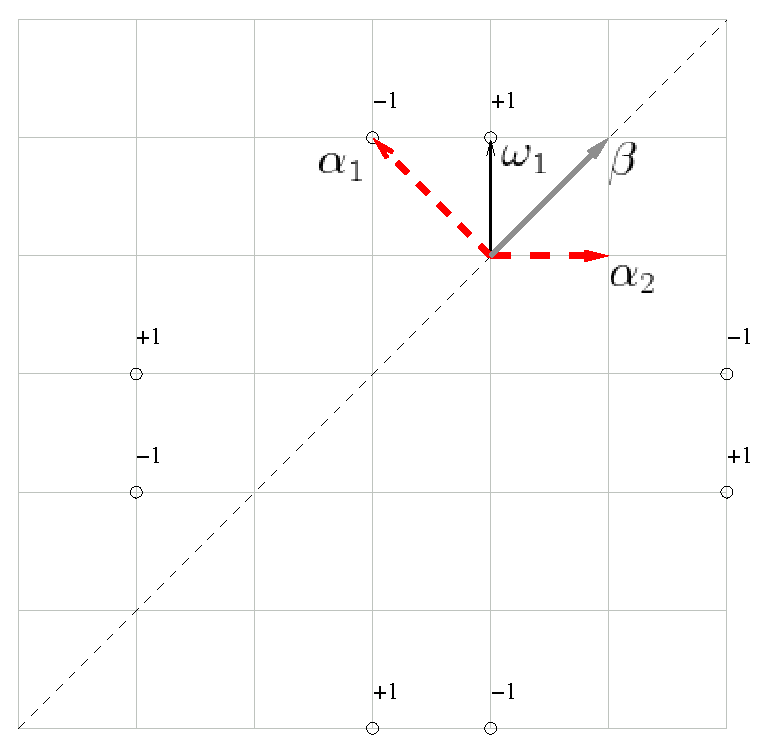
\includegraphics[width=60mm]{figures/figure1}
      \hfill
      \caption{Корни алгебр $B_{2},A_{1}$ и $\Psi ^{\omega_1  }$}
      \hfill
      \vspace{5mm}
      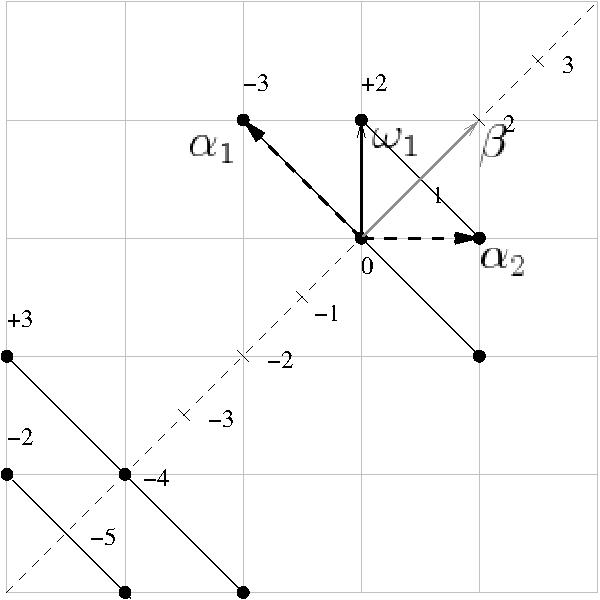
\includegraphics[width=60mm]{figures/figure2}
      \caption{Ортогональная подалгебра $\mathfrak{b}$ и размерности $\mathfrak{b}$-модулей}
    \end{multicols}
  \end{figure}
\end{frame}
\subsection{Аффинный пример}
\begin{frame}
  \begin{figure}[t]
    \vspace*{-0.5cm}
    \begin{multicols}{2}
      \hfill
      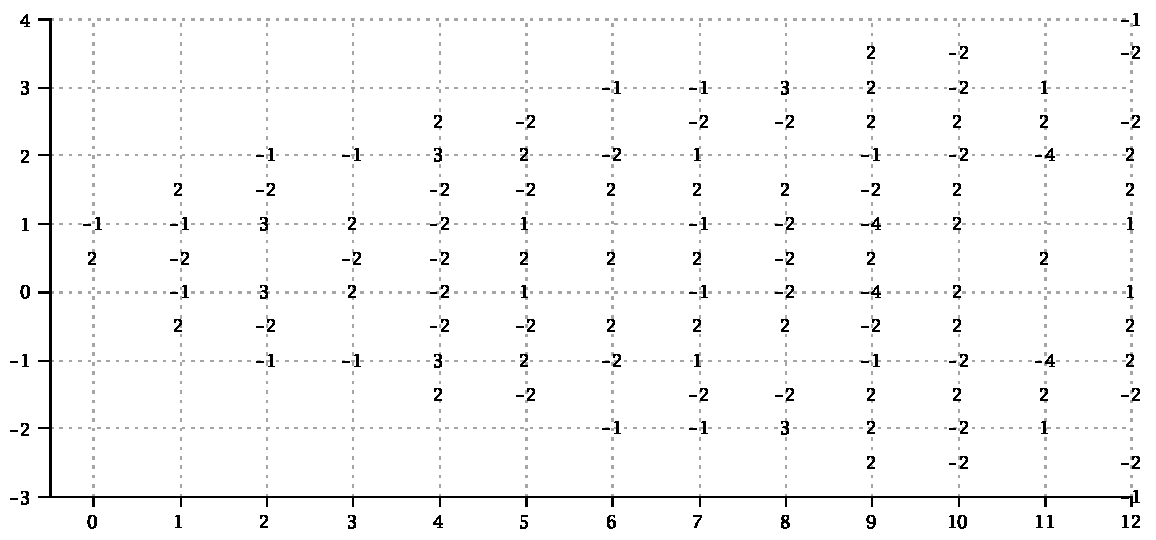
\includegraphics[width=60mm]{figures/figure10}
      \hfill
      \caption{$\Gamma_{\hat A_1\subset \hat B_2}$}
      \hfill
      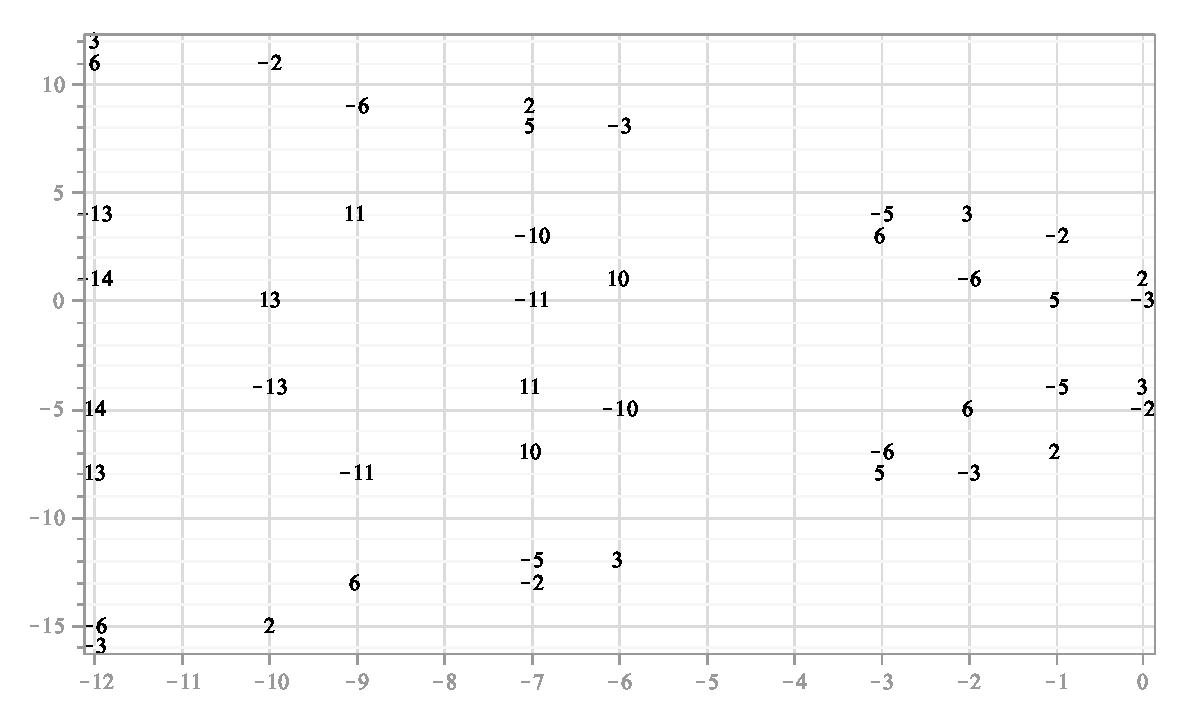
\includegraphics[width=60mm]{figures/figure12}
      \caption{ $\pi_{\hat A_{1}}\left( \Psi ^{\omega_1  }_{\hat B_{2}}\right)$}
    \end{multicols}
  \end{figure}
  \begin{figure}[b]
    \vspace*{-1.3cm}
    \centering
      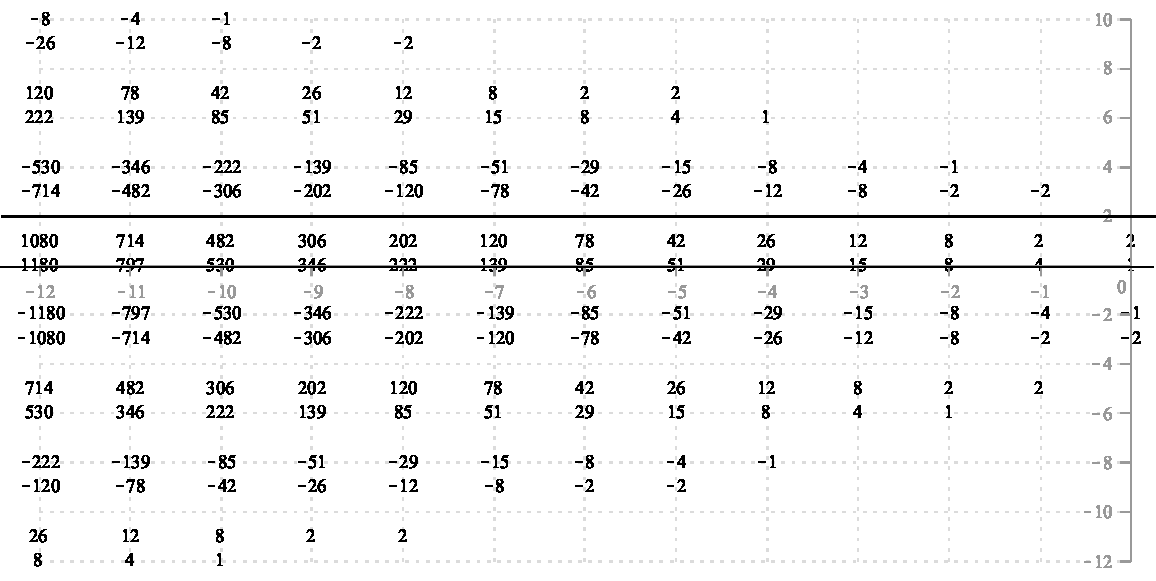
\includegraphics[width=100mm]{figures/figure13}
    \caption{Коэффициенты ветвления (со знаком) для $\hat A_1\subset \hat B_2$}
    \label{fig:2}
  \end{figure}
\end{frame}
\subsection{Выводы}
\begin{frame}
  \frametitle{Выводы к главе 2}
  \begin{itemize}
  \item Коэффициенты ветвления нужны для вычисления спектра возбуждений в WZNW-модели на торе
  \item Фунцкии ветвления дают статсумму coset-моделей
  \item Получена новая рекуррентная формула для коэффициентов ветвления, не требующая лишних вычислений
  \item Продемонстрирована эффективность алгоритма
  \end{itemize}
  \begin{figure}[b]
    \centering
      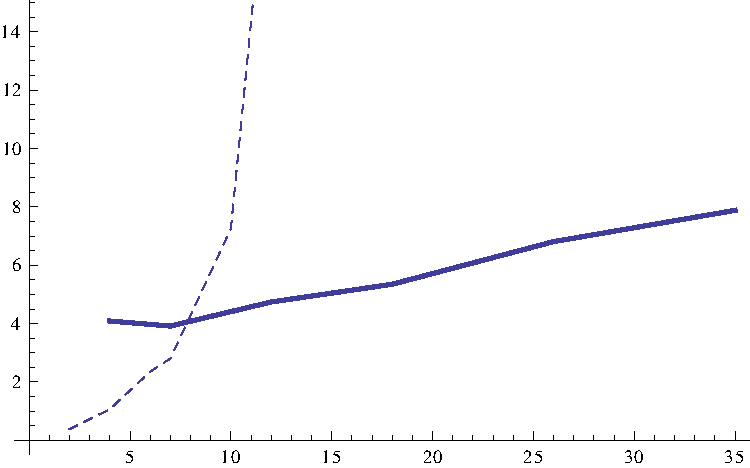
\includegraphics[width=50mm]{figures/branching-timing}
      \vspace{-0.3cm}
      \caption{Зависимость времени вычисления коэффициентов ветвления для вложения $B_{3}\to B_{4}$ от числа весов в $\bar C$. Пунктир -- традиционный алгоритм, сплошная линия -- наш алгоритм}
      \label{fig:branching}
  \end{figure}
\end{frame}
\section{Глава 3. Связь с обобщенной БГГ-резольвентой}
\begin{frame}
\frametitle{Связь с обобщенной резольвентой Бернштейна-Гельфанда-Гельфанда}
  Рассмотрим ситуацию без проекции ($\mathrm{rank}\af=\mathrm{rank}\gf$).
  \begin{equation*}
    M_{I}^{\mu _{\frak{a}_{\perp }}\left( u\right) }=U\left( \frak{g}\right)
    \otimes _{U\left( \frak{p}_{I}\right) }L_{\frak{a}_{\perp }}^{\mu _{\frak{a}%
        _{\perp }}\left( u\right) }\quad  \Delta _{\frak{a}_{\perp }}^{+}\sim  \Delta _{I}^{+}, \mbox{ где}\; I\subset S
  \end{equation*}
  Введем  $R_{I}:=\prod_{\alpha \in \Delta^{+}\setminus \Delta _{\pf_{I}}^{+}}\left( 1-e^{-\alpha }\right)^{\mathrm{mult}(\alpha )}$. Тогда
$\mathrm{ch}M_{I}^{\mu}=\frac{1}{R_{I}}\mathrm{ch}L_{\pf_{I}}^{\mu }$

  \begin{figure}[t]
    \vspace*{-0.2cm}
      \hfill
        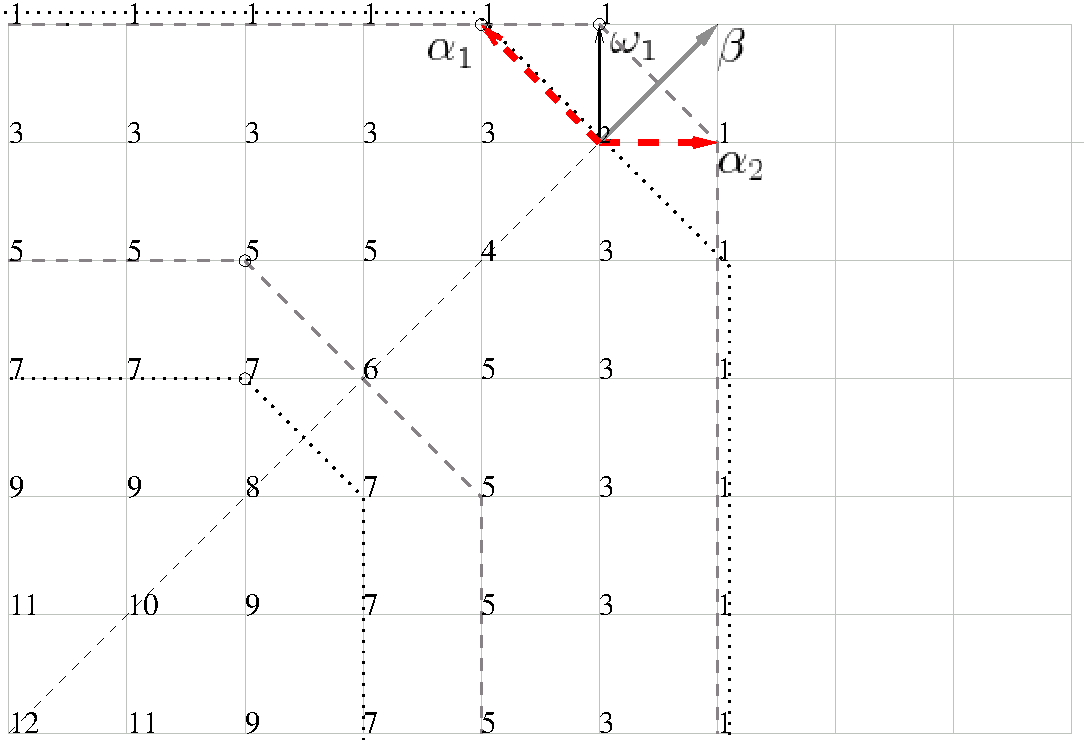
\includegraphics[width=60mm]{figures/B2_Gen_Verma_Decomp}
      \hfill
    \vspace*{-0.3cm}
      \caption{Вложение $A_{1}\oplus u(1) \subset B_{2}$ и обобщенные модули Верма.
        Пунктир -- с положительным знаком $\epsilon(u)$, точки --  с отрицательным.}
  \end{figure}
\end{frame}
\begin{frame}
  \frametitle{Точная последовательность}
  \begin{equation*}
    0\rightarrow M_{r}^{I}\overset{\delta _{r}}{\rightarrow }M_{r-1}^{I}\overset{%
      \delta _{r-1}}{\rightarrow }\ldots \overset{\delta _{1}}{\rightarrow }%
    M_{0}^{I}\overset{\varepsilon }{\rightarrow }L^{\mu }\rightarrow 0,
  \end{equation*}
  \begin{equation*}
    M_{k}^{I}=\bigoplus_{u\in U,\;\mathrm{length}\left( u\right)
      =k}M_{I}^{u\left( \mu +\rho \right) -\rho },\quad M_{0}^{I}=M_{I}^{\mu }
  \end{equation*}
  \vspace{-0.5cm}
  \begin{figure}[h!bt]
    \noindent\centering{
      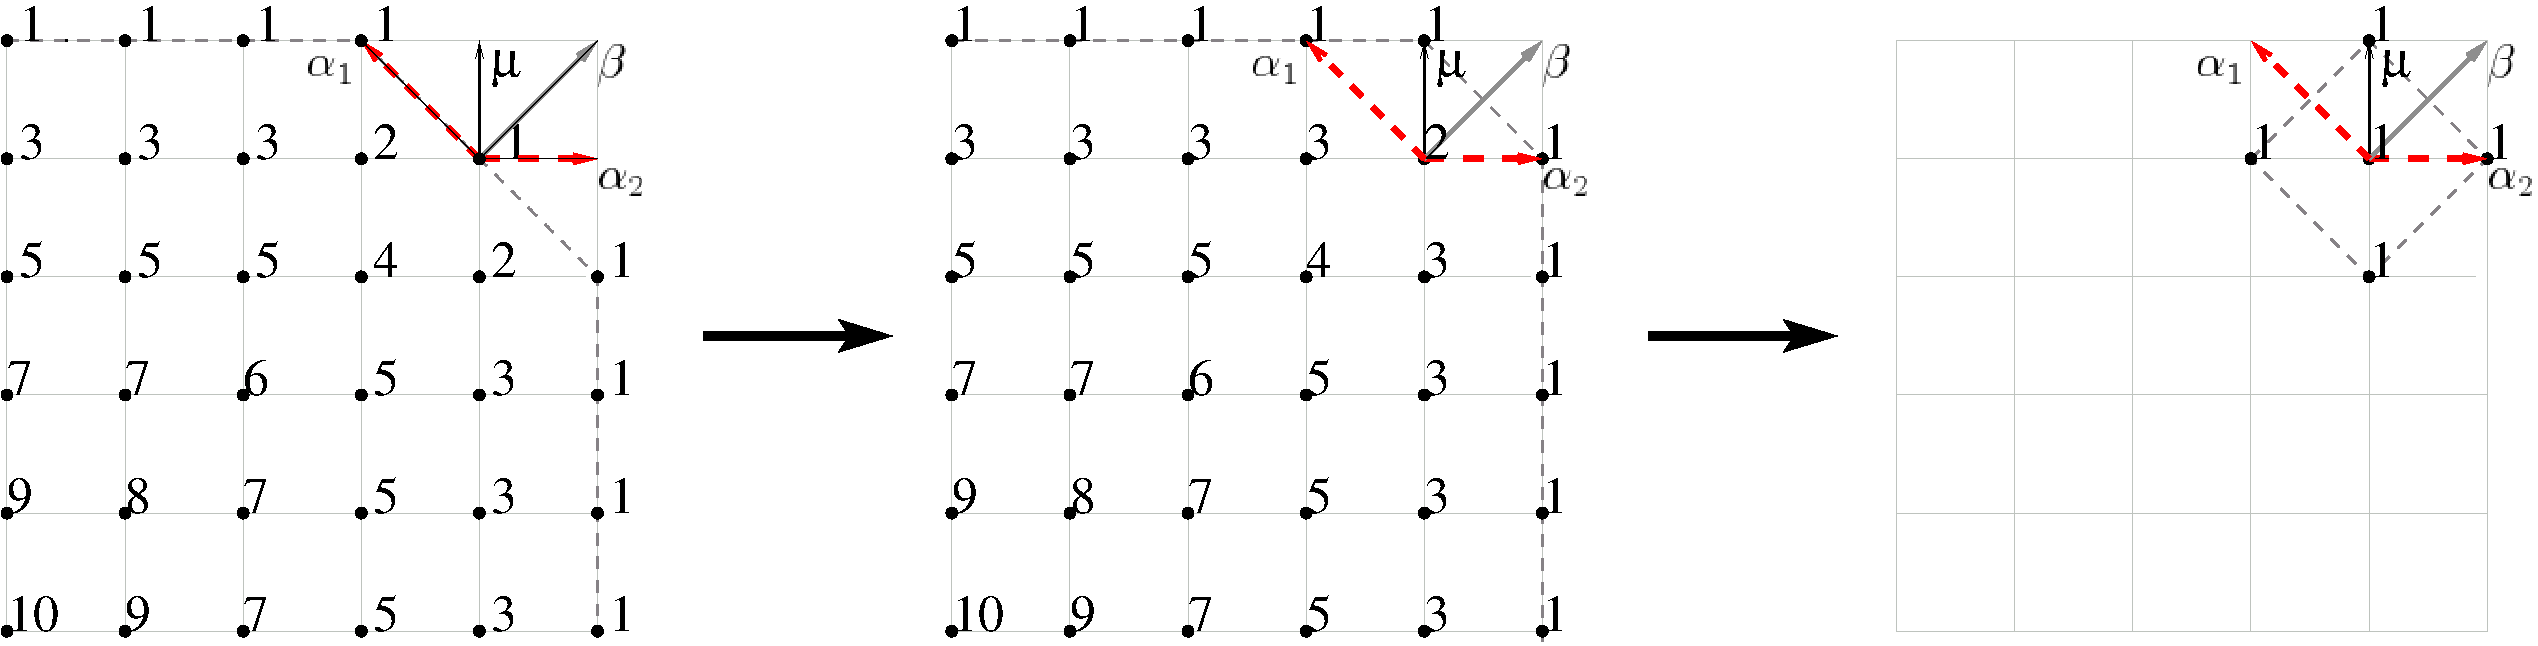
\includegraphics[width=120mm]{figures/B2_Exact}}
\vspace{-0.5cm}
    \caption{
      Резольвента модуля $L^{\omega_1}$.  Центральная часть точной последовательности
      $0 \to Im(\delta_2) \to \left( e^{\pi _{\aft}\left[ \mu \right] + \mathcal{D}_{\afb}}\mathrm{ch}M_{I}^{\pi _{\afb}\left[ \omega_1 \right] -
          \mathcal{D}_{\afb} }=M^{\omega_1}_{I}\right) \to
      L^{\omega_1}\to 0 $.  
    }
  \end{figure}
\end{frame}
\begin{frame}
  \frametitle{Выводы к главе 3}
  \begin{itemize}
  \item Показано, что использование веера вложения приводит к построению параболических модулей Верма
  \item Эти модули входят в точную последовательность обобщенной резольвентой Бернштейна-Гельфанда-Гельфанда
  \item То есть установлена связь ветвления с обобщенной БГГ-резольвентой
  \end{itemize}
\end{frame}
\section{Глава 4. Сплинты и ветвление}
\begin{frame}
  \frametitle{Сплинты}
  \begin{Def}
$\phi $ -- ``вложение'' $\Delta_{0}\hookrightarrow \Delta$:
$\phi (\gamma )=\phi (\alpha )+\phi (\beta )\quad  \forall \alpha ,\beta ,\gamma \in P_{0}: \gamma =\alpha+\beta.$

\end{Def}
$\phi$ индуцирует вложение формальных алгебр: ${\mathcal{E}}_0\hookrightarrow \mathcal{E}$ и  для ${\mathcal{E}}_i=\mathrm{Im}_{\phi}\left( {\mathcal{E}}_0\right)$ есть $\phi^{-1}:{\mathcal{E}}_i \longrightarrow {\mathcal{E}}_0$.

\begin{Def}
Корневая система $\Delta$ ``расщепляется'' на  $(\Delta _{1},\Delta _{2})$, если существует два вложения  $\phi _{1}:\Delta _{1}\hookrightarrow \Delta $ и $\phi _{2}:\Delta _{2}\hookrightarrow \Delta $, где (a) $\Delta $ -- несвязное объединение образов $\phi _{1}$ и $\phi _{2}$, и (b) ни ранг  $\Delta _{1}$, ни ранг  $\Delta _{2}$ не превосходит ранга $\Delta $.
\end{Def}
Пусть $\Delta _{1}=\Delta _{\af}$. $\Delta _{\sfr}:=\Delta_{2}=\Delta \setminus \Delta _{\af}$ определяет  веер вложения  $\Gamma _{\af\hookrightarrow \gf}$. 
$\prod_{\beta \in \Delta _{\sfr}^{+}}\left( 1-e^{-\beta }\right)
=-\sum_{\gamma \in P}s(\gamma )e^{-\gamma }$

$\Psi _{\gf}^{\left( \mu \right) }=e^{-\rho}\sum_{w\in W_{\af}}w\circ \left(
e^{\rho _{\af}}\phi_{2}\left(\Psi ^{\widetilde{\mu }+\rho _{\sfr}}\right)\right) \quad \mu=\sum m_{k}\omega ^{k},\;\widetilde{\mu }=\sum m_{k}\omega _{\sfr}^{k}$

\end{frame}
\begin{frame}
  \frametitle{Пример}
  \vspace{-0.5cm}
\begin{figure}[h!bt]
  \hspace*{-1.2cm}

   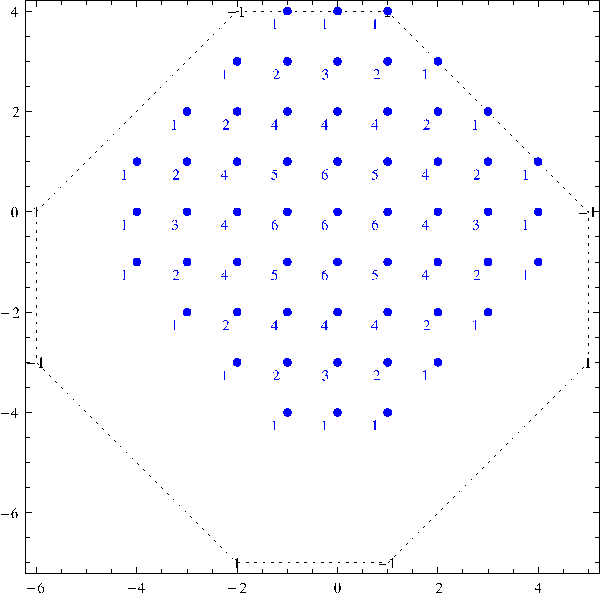
\includegraphics[width=50mm]{figures/b2}
   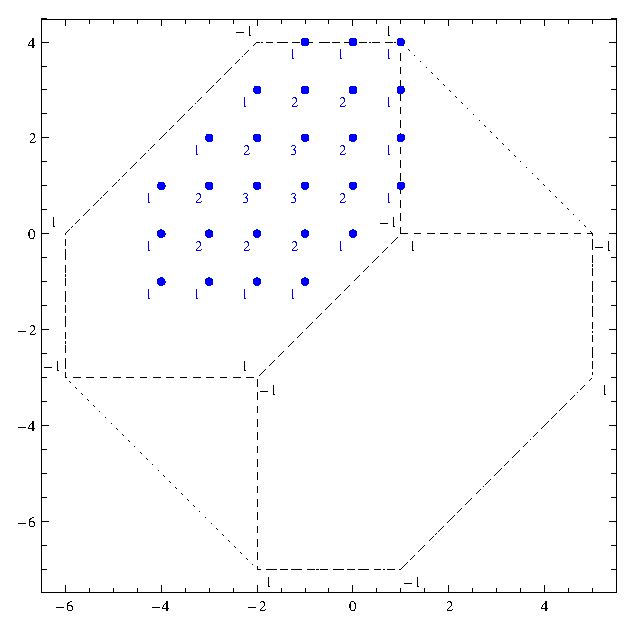
\includegraphics[width=50mm]{figures/b2-a2-a1}
  \caption{Веса  $L^{[3,2]}_{B_{2}}$  с кратностями показаны слева. Короткий пунктир -- контур сингулярного элемента. Справа -- разложение сингулярного элемента $\Psi_{B_{2}}(L^{[3,2]}_{B_{2}})$ в сумму образов сингулярных элементов $\Psi_{A_{2}}(L^{[3,2]})$ (длинный пунктир). Кратности $L^{[3,2]}_{A_{2}}$ =  коэффициентам ветвления $L^{[3,2]}_{B_{2}\downarrow A_{1}\oplus u(1)}$.}

 \label{fig:b2_splint}
\end{figure}

\end{frame}

\subsection{$G_2$}
\begin{frame}
  
  \begin{figure}[h!bt]
    \noindent\centering{
   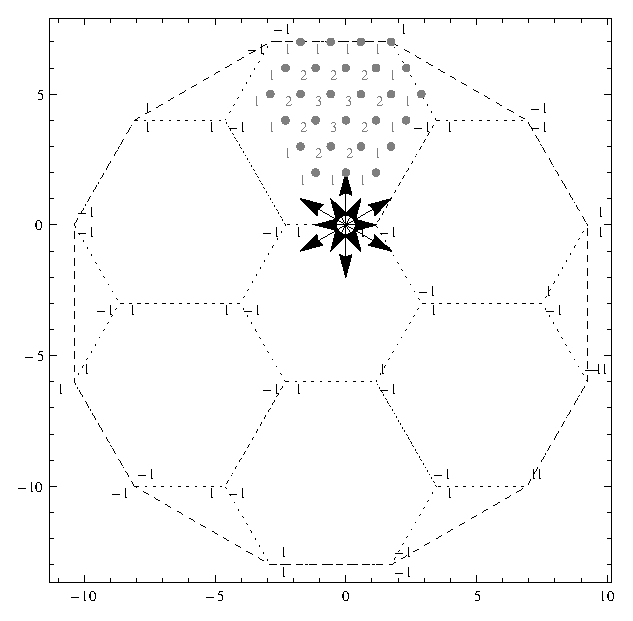
\includegraphics[width=65mm]{figures/g2}
  }

  \caption{Орбита группы Вейля  (длинный пунктир) для  $\Psi_{G_{2}}(L^{[3,2]})$ и его разложение в сумму образов сингулярных элементов модулей  $A_{2}$ (короткий). Кратности весов  $L^{[3,2]}_{A_{2}}$ совпадают с коэффициентами ветвления $L^{[3,2]}_{G_{2}\downarrow A_{2}}$.}


 \label{fig:g2_splint}
\end{figure}

\end{frame}

\subsection{Аффинные алгебры}
\begin{frame}
Аффинное расширение $\afh\subset\gfh$. Так как $\mathrm{rank}\gf\leq\mathrm{rank} \af+\mathrm{rank}\sfr$, для знаменателей Вейля 
\begin{multline*}
\prod_{\alpha\in\hat{\Delta}^{+}_{1}}(1-e^{-\alpha})^{\mathrm{mult}(\alpha)}\prod_{\beta\in\hat{\Delta}^{+}_{2}}(1-e^{\phi\circ \beta})^{\mathrm{mult}(\beta)}=\\
\prod_{\gamma\in\hat{\Delta}^{+}}(1-e^{-\gamma})^{\mathrm{mult}(\gamma)}\prod_{n=0}^{\infty}(1-e^{-n\delta})^{\mathrm{rank}\af+\mathrm{rank}\sfr-\mathrm{rank}\gf}
\end{multline*}
 $$\Theta^{(\gfh)}_{\widehat{\lambda}=(\lambda,k,0)}(\tau,z)=\sum_{\xi\in Q_{\gf}+\frac{\lambda}{k}}e^{2\pi i k \left(\frac{1}{2} (\xi,\xi) \tau + (\xi,z)\right)}$$
Соотношение, связывающее тета-функции алгебр $\gfh,\hat\sfr,\afh$:
\begin{multline*}
  \left(\sum_{v\in W_{\af}}\epsilon(v) \Theta^{(\afh)}_{v\rho_{\af}}(\tau,z)\right)
  \cdot \left(\sum_{u\in W_{\sfr}}\epsilon(u) \Theta^{(\hat{\sfr})}_{\phi\circ(u\rho_{\sfr})}(\tau,z)\right)= \\
  \left(\sum_{w\in W}\epsilon(w) \Theta^{(\gfh)}_{w\rho_{\gf}}(\tau,z)\right)
\end{multline*}
\end{frame}
\begin{frame}
  \frametitle{Ветвление на конечномерные подалгебры}

Рассмотрим ветвление модуля $\gfh$ на модули $\gf$
\begin{equation*}
  \label{eq:149}
\mathrm{ch}L^{\hat{\mu}}_{\gfh}=\sum_{n=0}^{\infty}e^{-n\delta} \sum_{\nu\in P} b^{(\hat{\mu})}_{\nu}(n) \mathrm{ch} L^{\nu}_{\gf} \quad m^{(\hat{\mu})}_{\hat{\nu}=(\nu,k,n)}=\sum_{\xi\in P}
b^{(\hat{\mu})}_{\xi}(n) m^{(\xi)}_{\nu}
\end{equation*}
Введем $b^{(\hat{\mu})}_{\nu}(q):=\sum_{n=0}^{\infty} b^{(\hat{\mu})}_{\nu}(n) q^{n}$, они связаны с  $q$-размерностью \\ $\mathrm{dim}_{q}L^{\hat \mu}_{\gfh}=\sum_{n=0}^{\infty}q^{n}\sum_{\nu\in P} b^{(\hat \mu)}_{\nu}(n) \mathrm{dim }L^{\nu}_{\gf}=\sum_{\nu\in P}b^{(\hat\mu)}_{\nu}(q) \mathrm{dim} L^{\nu}_{\gf}$.

 $ \sigma^{(\hat{\mu})}_{\nu}(q) = \sum_{\xi\in P} m^{(\xi)}_{\nu} b^{(\hat{\mu})}_{\xi}(q)$.

Введем порядок на множестве весов $\xi$ следующим образом:
припишем весу  $\xi$ значение  $(\rho,\xi)$ и упорядочим веса по этим значениям. Тогда  $$\sigma(q)=M b(q)\quad b(q)=M^{-1}\sigma(q)$$
  $\sigma(q)$ и  $b(q)$ -- бесконечные векторы струнных функций и функций ветвления. Матрица $M$ содержит кратности весов в  $\gf$-модулях. Обратная матрица $M^{-1}$ содержит рекуррентные соотношения на кратности весов.
\end{frame}
\begin{frame}
    \frametitle{Матричные соотношения для сплинтов}
Рассмотрим ветвление модулей  $\gfh$ на модули $\af$ в предположении существовании сплинта
$\Delta^{+}_{\gf}=\Delta^{+}_{\af}\cup \phi(\Delta^{+}_{\sfr})$.
Разложим  $\gf$-модули на 
$\af$-модули используя свойство сплинта:
\begin{multline}
  \label{eq:125}
  \mathrm{ch}L^{\hat{\mu}}_{\gfh}=
\sum_{n=0}^{\infty}e^{-n\delta} \sum_{\nu\in P_{\af}} b^{(\hat{\mu})}_{(\gfh\downarrow\af)\nu}(n) \mathrm{ch} L^{\nu}_{\af}=\\
\sum_{n=0}^{\infty} e^{-n\delta} \sum_{\nu\in P} b^{(\hat{\mu})}_{(\gfh\downarrow\gf )\nu}(n) \sum_{\xi\in P_{\af}} b^{(\nu)}_{(\gf\downarrow \af) \xi}\mathrm{ch} L^{\xi}_{\af}=\\
=\sum_{n=0}^{\infty} e^{-n\delta} \sum_{\nu\in P} b^{(\hat{\mu})}_{(\gfh\downarrow\gf )\nu}(n) \sum_{\xi\in P_{\af}} M^{\widetilde{\nu}}_{  \widetilde{\nu}-\phi^{-1}( \nu-\xi )}\mathrm{ch} L^{\xi}_{\af}
\end{multline}
  Матричное соотношение выполняется для функций ветвления $b_{(\gfh\downarrow\af)}(q)= M_{\sfr}\;
b_{(\gfh\downarrow\gf)}(q)$ и мы можем написать
$\sigma(q)=M_{\af}\; b_{(\gfh\downarrow\af)}(q)$.  Зная коэффициенты ветвления для вложения $\gf\subset\gfh$  сразу получаем (градуированные) функции ветвления для вложения $\af\subset \gfh$.
\end{frame}
\subsection{Выводы}
\begin{frame}
  \frametitle{Выводы к главе 4}
  \begin{itemize}
  \item Проанализирована связь расщепления с веером вложения
  \item Доказано, что расщепление корневой системы приводит к совпадению коэффициентов ветвления с кратностями весов
  \item Для аффинных алгебр получены новые соотношения на тета-функции
  \item Показано, что существование сплинта ведет к матричным соотношениям между функциями ветвления 
  \end{itemize}
\end{frame}
\section{Глава 5. Приложения}
\label{sec:applications}

\subsection{Эволюция Шрамма-Лёвнера и coset-модели}
\label{sec:SLE}
\begin{frame}
  \frametitle{Эволюция Шрамма-Лёвнера}
  \begin{Def}
    {\it Эволюция Шрамма-Лёвнера} на верхней полуплоскости  $\mathbb{H}$ -- это стохастический процесс, удовлетворяющий уравнению
    \begin{equation*}
      \frac{\partial g_t(z)}{\partial t} = \frac{ 2}{g_t(z)-\sqrt{\kappa}\xi_{t}} \quad \text{or} \quad       d w _{t}= \frac{2dt}{w_{t} }-\sqrt{\kappa}\xi_{t}
    \end{equation*}
  \end{Def}
  Конформно-инвариантная мера на траекториях $\gamma_{t}$ in $\mathbb{H}$.
  \begin{figure}[h]
    \begin{multicols}{2}
      \hfill
      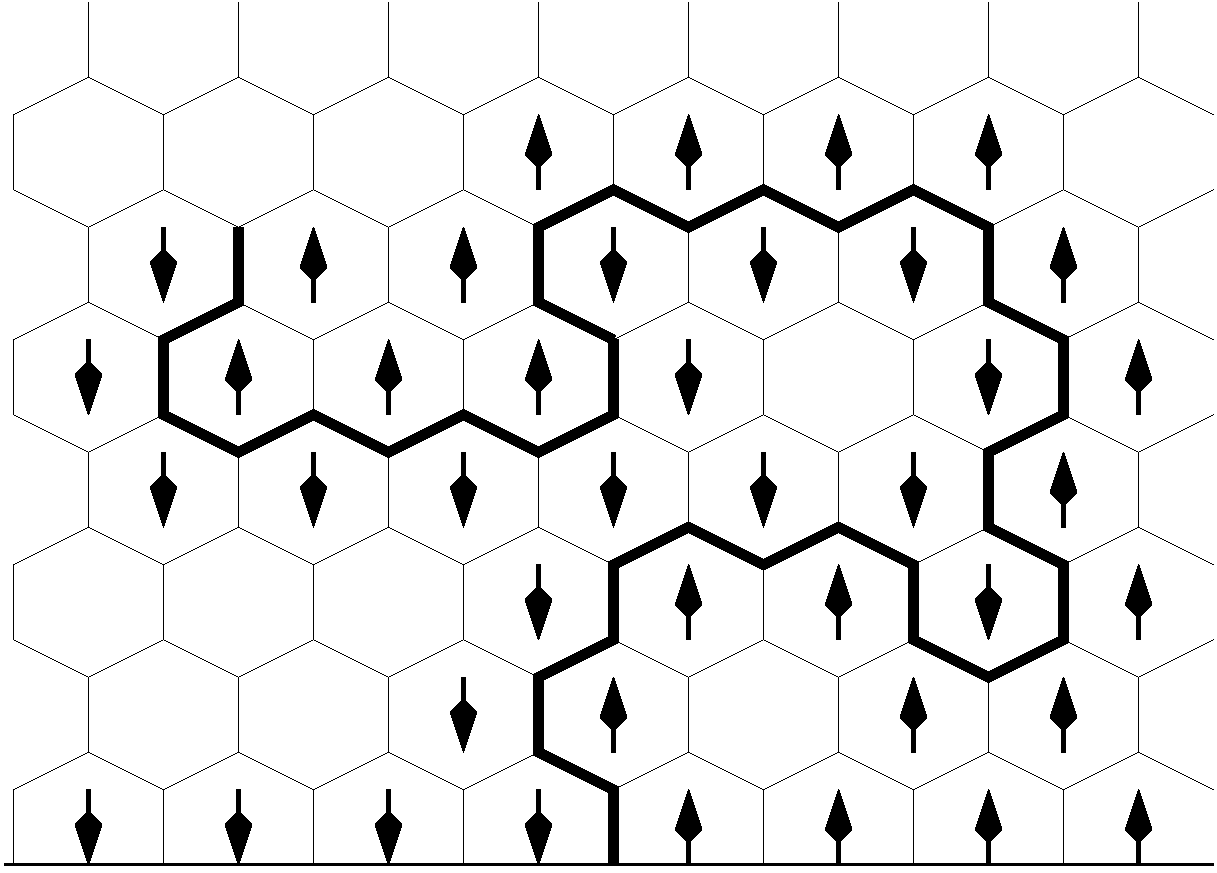
\includegraphics[height=25mm]{figures/explore.pdf}
      \vspace{-0.2cm}
      \caption{Эволюция Шрамма-Лёвнера -- непрерывный предел интерфейсов}
      \label{fig:sle}
      \hfill
      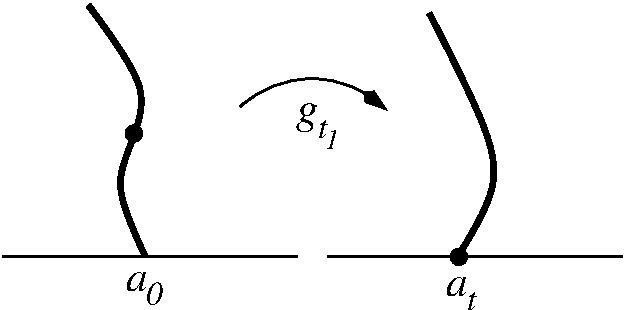
\includegraphics[width=50mm]{figures/loewner.pdf}
      \caption{Конформное отображение}
      \label{fig:sle}
    \end{multicols}

  \end{figure}
\end{frame}

\begin{frame}
  \frametitle{Стохастические наблюдаемые и корреляторы в CFT}
      \vspace{-0.2cm}
  Рассмотрим решеточную наблюдаемую $\mathcal{O}$, тогда
  \begin{equation*}
    \prec \mathcal{O} \succ_{\mathbb{H}}=\mathbb{E}\left[\prec\mathcal{O}\succ_{\gamma_{t}}\right]=\sum_{\gamma_{t}} P\left[C_{\gamma_{t}}\right] \prec \mathcal{O} \succ_{\gamma_{t}}
  \end{equation*}
  $\prec \mathcal{O} \succ_{\mathbb{H}}$ не зависит от $t$, следовательно $\prec\mathcal{O}\succ_{\gamma_{t}}$ -- мартингал.

  Непрерывный предел в критической точке дается корреляционной функцией в конформной теории поля
  \begin{equation*}
    \prec \mathcal{O} \succ_{\mathbb{H}_{t}}\to \mathcal{F}(\left\{z_{i}\right\})_{\mathbb{H}_{t}}=
    \frac{\left< \mathcal{O}(\{z_{i}\})\phi(z_{t})\phi^{\dagger}(\infty)\right>_{\mathbb{H}_{t}}}{\left<\phi(z_{t})\phi^{\dagger}(\infty)\right>_{\mathbb{H}_{t}}}=
    \frac{\left< ^{g_{t}}\mathcal{O}\phi(\xi_{t})\phi^{\dagger}(\infty)\right>_{\mathbb{H}}}{\left<\phi(z_{t})\phi^{\dagger}(\infty)\right>_{\mathbb{H}}}
  \end{equation*}
  Здесь $\phi$ -- оператор изменения граничных условий.


  После конформного отображения $w(z):\mathbb{H}\setminus\gamma_{t}\to \mathbb{H}$
  \begin{equation*}
    \mathcal{F}(\left\{z_{i}\right\})_{\mathbb{H}_{t}}=\prod \left(\frac{\partial w(z_{i})}{\partial z_{i}}\right)^{h_{\lambda_i}} 
    \prod \left(\frac{\partial \bar w(\bar z_{i})}{\partial \bar z_{i}}\right)^{h_{\lambda^{*}_i}}
        \mathcal{F}(\left\{w_{i}, \bar w_{i}\right\})_{\mathbb{H}}
  \end{equation*}
  При переходе от  $t$ к $t+dt$ первый сомножитель дает $-\frac{2h_{\lambda_{i}}}{w_{i}^{2}}\left(\frac{\partial w_{i}}{\partial z_{i}}\right)^{h_{\lambda_{i}}}$.
\end{frame}
\begin{frame}
  \frametitle{Мартингалы стохастического процесса}
   Поля преобразуются так:
   \begin{itemize}
   \item   Минимальные модели -- только конформные преобразования
     $d\phi_{\lambda_{i}}(w_{i}) = \mathcal{G}_{i}\phi_{\lambda_{i}}(w_{i})=\left(\frac{2dt}{w_{i}}-\sqrt{\kappa} d\xi_{t}\right) \partial_{w_{i}}\phi_{\lambda_{i}}(w_{i})$
   \item WZNW-модели -- калибровочные преобразования
  \begin{equation*}
    \mathcal{G}_{i}=\left(\frac{2dt}{w_{i}}-\sqrt{\kappa} d\xi_{t}\right) \partial_{w_{i}}+\frac{\sqrt{\tau}}{w_{i}}\left(\sum_{a=1}^{\mathrm{dim} \gf}\left(d \theta ^{a} t^{a}_{i}\right)\right)
  \end{equation*}
\item coset-модели $\mathcal{G}_{i}=\left(\frac{2dt}{w_{i}}-\sqrt{\kappa} d\xi_{t}\right) \partial_{w_{i}}+\frac{\sqrt{\tau}}{w_{i}}\left(\sum_{a:\mathcal{K}(t^{a},\tilde{t}^{b})=0}\left(d \theta ^{a} t^{a}_{i}\right)\right)$.
Разрешили случайные блуждания в направлении $\perp \af$.
   \end{itemize}

  Верно равенство
$    \mathbb{E}\left[\prec\mathcal{O}\succ_{\gamma_{t}}\right]=    \mathbb{E}\left[\prec\mathcal{O}\succ_{\gamma_{t+dt}}\right], \quad \mathbb{E}\left[d \prec\mathcal{O}\succ_{\gamma_{t}}\right]=0
$
  Используя формулу Ито, получаем $0 =$
  \begin{multline}
    \hspace{-0.5cm}
    \left(\prod_{i=1}^{2N}\left(\frac{\partial w_{i}}{\partial z_{i}}\right)^{-h_{i}}\right)\mathbb{E}\left[d 
      \mathcal{F}_{\mathbb{H}_{t}}\right]=
    \left(-\sum_{i=1}^{2N}\frac{2h_{i}dt}{w_{i}^{2}}+\mathbb{E}\left[\sum_{i=1}^{2N}\mathcal{G}_{i}+\frac{1}{2}
        \sum_{i,j}\mathcal{G}_{i}\mathcal{G}_{j}\right]\right)\mathcal{F}_{\mathbb{H}} = 0
  \end{multline}
%%    Подставляем явный вид конформного преобразования полей и получаем равенство
%%    \begin{equation*}
%%      \left( \sum_{i}\left[-\frac{2h_{i}}{w_{i}^{2}} +\frac{2}{w_{i}}\partial_{w_{i}}\right]+\frac{\kappa}{2}\sum_{i,j}\partial_{w_{i}} \partial_{w_{j}}\right)\mathcal{F}(\left\{z_{i}\right\})=0
%%    \end{equation*}
%%  
%%    Можно переписать в виде соотношений на оператор смены граничных условий $\phi$:
%%    \begin{equation*}
%%      (L_{-2}-\frac{\kappa}{2}L_{-1}^{2})\phi=0 \Longrightarrow \phi \left|0\right>  \text{has level 2 null state}, \phi\sim \phi_{1,2} \;\text{or}\; \phi_{2,1}
%%    \end{equation*}
%%  
\end{frame}
%%  \begin{frame}
%%    \frametitle{Эволюция Шрамма-Лёвнера на факторпространстве}
%%      В $\gf\oplus \af$ WZNW-модели генератор преобразования примарного поля при эволюции от $t$ до $t+dt$
%%    \begin{equation*}
%%      \mathcal{G}_{i}=\left(\frac{2dt}{w_{i}}-\sqrt{\kappa} d\xi_{t}\right) \partial_{w_{i}}+\frac{\sqrt{\tau}}{w_{i}}\left(\sum_{a=1}^{\mathrm{dim} \gf}\left(d \theta ^{a} t^{a}_{i}\right)+\sum_{b=1}^{\mathrm{dim} \af}\left(d \tilde{\theta} ^{b} \tilde{t}^{b}_{i}\right)\right)
%%    \end{equation*}
%%  %%    \begin{equation*}
%%  %%      \mathcal{G}_{i}^{L,R}=\left(\frac{2dt}{w_{i}}-\sqrt{\kappa} d\xi_{t}\right) \partial_{w_{i}}+\frac{\sqrt{\tau}}{w_{i}}\left(\sum_{a=1}^{\mathrm{dim} \gf}\left(d \theta ^{a} t^{a}_{i}\right)\pm\sum_{b=1}^{\mathrm{dim} \af}\left(d \tilde{\theta} ^{b} \tilde{t}^{b}_{i}\right)\right)
%%  %%    \end{equation*}
%%  
%%    Условие на мартингал
%%    \begin{equation*}
%%      \left(-2 \mathcal{L}_{-2}+\frac{1}{2}\kappa \mathcal{L}_{-1}^{2}+\frac{\tau}{2}\left( \sum_{a} \mathcal{J}^{a}_{-1} \mathcal{J}^{a}_{-1}-
%%          \sum_{b}\tilde{\mathcal{J}}^{b}_{-1} \tilde{\mathcal{J}}^{b}_{-1}\right)\right)        \mathcal{F}_{\mathbb{H}}=0
%%    \end{equation*}
%%  
%%  перепишем в виде требования что поле
%%  \begin{equation*}
%%    \psi=\left(-2L_{-2}+\frac{1}{2}\kappa L_{-1}^{2}+\frac{1}{2}\tau \left(\sum_{a=1}^{\mathrm{dim}\gf}J^{a}_{-1}J^{a}_{-1}-\sum_{b=1}^{\mathrm{dim}\af}\tilde{J}^{b}_{-1}\tilde{J}^{b}_{-1}\right)\right) \phi_{(\Lambda,\Gamma)}
%%  \end{equation*}
%%  является сингулярным на уровне два.
%%  \end{frame}
%%  
%%  

\begin{frame}
  \frametitle{Парафермионы и минимальные модели в coset-конструкции}
$|\psi>=\left(-2L_{-2}+\frac{1}{2}\kappa L_{-1}^{2}+\frac{1}{2}\tau \left(\displaystyle{\sum_{a=1}^{\dim\gf}}J^{a}_{-1}J^{a}_{-1}-\displaystyle{\sum_{b=1}^{\dim\af}}\tilde{J}^{b}_{-1}\tilde{J}^{b}_{-1}\right)\right) 
\varphi(0)|0>$

  $\mathbb{Z}(N)$-парафермионы эквивалентны $SU(2)_{N}/U(1)$ coset-теории.
  
  Парафермионное поле раскладывается в произведение
  \begin{equation*}
    \Phi^{j}=\phi_{j}(z) \exp\left( -i \frac{j}{\sqrt{N}}\phi(z)\right)
  \end{equation*}
  где $\phi_{j}(z)$ -- поле $SU(2)$-WZNW модели со спином $j$, $\phi(z)$ -- $U(1)$ бозонное поле.
  
  Парафермионный ток $ \Psi^{\pm}=\frac{1}{\sqrt{N}} J^{\pm}\exp\left(\mp i \frac{1}{\sqrt{N}}\phi(z)\right)$
%%  Its action in terms of primary fields of $su(2)\oplus u(1)$ WZNW-model is equivalent to $J^{\pm}\pm \tilde{J}^{\pm}$.

  Условие на мартингалы принимает вид
  \begin{equation*}
    \left(-2 L_{-2}+\frac{\kappa}{2}L_{-1}^{2}+\frac{\tau}{2}\left[\Psi^{+}_{-1}\Psi^{-}_{-1}+\Psi^{-}_{-1}\Psi^{+}_{-1}\right]\right) \left|\Phi\right>=0
  \end{equation*}
  что совпадает с результатом Santachiara [arXiv:0705.2749].
\end{frame}

\subsection{Программа Affine.m}
\label{sec:-affine.m}

\begin{frame}[fragile]
  \begin{lstlisting}[mathescape=true]
stringFunctions[$\hat A_2$,{1,1,2}]
{{0, 0, 4}, 
$2 q + 10 q^2 + 40 q^3 + 133 q^4 + 398 q^5 + 1084 q^6 + 2760 q^7 + 6632 q^8 + 15214 q^9 + 33508 q^{10}$}, 
{{0, 3, 1}, 
$2 q + 12 q^2 + 49 q^3 + 166 q^4 + 494 q^5 + 1340 q^6 + 3387 q^7 + 8086 q^8 + 18415 q^9 + 40302 q^{10}$}, 
{{1, 1, 2}, 
$1 + 6 q + 27 q^2 + 96 q^3 + 298 q^4 + 836 q^5 + 2173 q^6 + 5310 q^7 + 12341 q^8 + 27486 q^9 + 59029 q^{10}$}, 
{{2, 2, 0}, 
$1 + 8 q + 35 q^2 + 124 q^3 + 379 q^4 + 1052 q^5 + 2700 q^6 + 6536 q^7 + 15047 q^8 + 33248 q^9 + 70877 q^{10}$}, 
{{3, 0, 1}, 
$2 + 12 q + 49 q^2 + 166 q^3 + 494 q^4 + 1340 q^5 + 3387 q^6 + 8086 q^7 + 18415 q^8 + 40302 q^9 + 85226 q^{10}$}
\end{lstlisting}

\begin{lstlisting}[mathescape=true]
vm=makeVermaModule[$B_{2}$][{2,1}];
pm=makeParabolicVermaModule[$B_{2}$][weight[$B_{2}$][2,1],{1}];
im=makeIrreducibleModule[$B_{2}$][2,1];
GraphicsRow[textPlot/@{im,vm,pm}]
$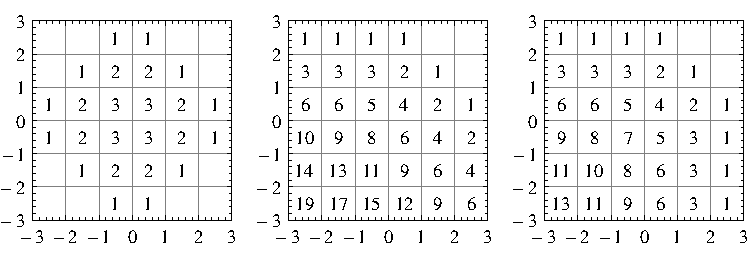
\includegraphics[width=100mm]{figures/irrep-verma-pverma.pdf}$
\end{lstlisting}

\end{frame}

\subsection{Выводы}
\begin{frame}
  \frametitle{Выводы к главе 5}
  \begin{itemize}
  \item Предложено обобщение эволюции Шрамма-Лёвнера, которое соответствует coset-моделям конформной теории поля
  \item Это обобщение интересно с точки зрения интегрируемых деформаций вне критической точки
  \item Получены условия на оператор смены граничных условий, которые совпадают с результатами Raul Santachiara
  \item Классификация операторов изменения граничных условий связана со структурой сингулярных элементов
  \item Реализован пакет {\bf Affine.m} для вычислений в теории представлений в системе {\it Mathematica}
  \item Этот пакет использовался для подготовки большинства примеров в данной работе
  \end{itemize}
\end{frame}
\section{Заключение}


\begin{frame}
  \frametitle{Основные результаты работы}
\begin{itemize}
\item Из разложения сингулярных элементов получены новые рекуррентные соотношения на коэффициенты ветвления представлений аффинных алгебр Ли на представления произвольных редуктивных подалгебр
\item Показана связь процедуры редукции с обобщенной резольвентой Бернштейна-Гельфанда-Гельфанда
\item Выявлена связь расщепления корневой системы алгебры с разложением сингулярных элементов модулей алгебры в комбинацию сингулярных элементов модулей подалгебр
\item Показано, что наличие расщепления существенно упрощает вычисление коэффициентов ветвления и ведет к новым соотношениям на функции ветвления
\item Предложено обобщение стохастического процесса Шрамма-Лёвнера на случай калибровочных теорий, соответствующих coset-моделям
\item Реализован пакет {\bf Affine.m} для теории представлений
\end{itemize}

\end{frame}

\begin{frame}
  \frametitle{Публикации в журналах}
  \begin{itemize}
  \item
    V.~{Lyakhovsky} and A.~{Nazarov}, ``{Recursive algorithm and branching for
      nonmaximal embeddings},''
    \href{http://dx.doi.org/10.1088/1751-8113/44/7/075205}{{\em Journal of
        Physics A: Mathematical and Theoretical} {\bf 44} (2011) no.~7, 075205},
    \href{http://arxiv.org/abs/1007.0318}{{\tt arXiv:1007.0318 [math.RT]}}.

  \item
    V.~{Lyakhovsky} and A.~{Nazarov}, ``{Recursive properties of branching and BGG
      resolution},'' \href{http://dx.doi.org/10.1007/s11232-011-0132-9}{{\em
        Theoretical and Mathematical Physics} {\bf 169} (2011) no.~2, 1551--1560},
    \href{http://arxiv.org/abs/1102.1702}{{\tt arXiv:1102.1702 [math.RT]}}.

  \item
    V.~{Laykhovsky} and A.~{Nazarov}, ``{Fan, splint and branching rules},'' {\em
      Zapiski Nauchnykh Seminarov POMI} {\bf 398} (2012)  162--179,
    \href{http://arxiv.org/abs/1111.6787}{{\tt arXiv:1111.6787 [math.RT]}}.

  \item
    A.~{Nazarov}, ``{Algebraic properties of CFT coset construction and
      Schramm-Loewner evolution},'' {\em Journal of Physics: Conference Series}
    {\bf 343} (2012) no.~1, 012085, \href{http://arxiv.org/abs/1112.4354}{{\tt
        arXiv:1112.4354 [math-ph]}}.
%    \url{http://stacks.iop.org/1742-6596/343/i=1/a=012085}.
  \item
    A.~{Nazarov}, ``{SLE martingales in coset conformal field theory},''  {\em
      JETP Letters} {\bf 96}, 1,  (2012)  162--179,
    \href{http://arxiv.org/abs/1205.6104}{{\tt arXiv:1205.6104 [math-ph]}}.


  \end{itemize}
\end{frame}
\begin{frame}
  \frametitle{Доклады и препринты}
  \begin{itemize}
  \item
    A.~Nazarov, ``Comparison of algorithms for construction of representations of
    Lie algebras,'' in {\em Physics and Progress}, Physics and Progress, SPbSU.
     2008.

  \item
    A.~Nazarov, ``Computational tools for representation theory of affine lie
    algebras,'' in {\em second Workshop on Advanced Computer Simulation Methods
      for Junior scientists}, ACSM, EIMI.
     2009.

  \item
    V.~{Lyakhovsky} and A.~{Nazarov}, ``{Branching functions generated by the
      injection fan for Lie algebras. (The role of BGG-resolvent)},'' in 
    {\em Models in Quantum Field Theory 2010} 
    % \url{http://hep.niif.spbu.ru/conf/mktp2010/}.

  \item
    V.~{Laykhovsky} and A.~{Nazarov}, ``{On affine extension of splint root
      systems},'' {\em To appear in PEPAN Letters}  ,
    \href{http://arxiv.org/abs/1204.1855}{{\tt arXiv:1204.1855 [math.RT]}}.
  \item
    A.~{Nazarov}, ``{Affine.m - Mathematica package for computations in
      representation theory of finite-dimensional and affine Lie algebras},'' {\em
    To appear in Computer Physics Communications} (2012)  , \href{http://arxiv.org/abs/1107.4681}{{\tt
        arXiv:1107.4681 [math.RT]}}.
  \end{itemize}
\end{frame}

\begin{frame}[c]
  \begin{center}
  \Large{Спасибо за внимание!}    
  \end{center}

\end{frame}

\end{document}
